% Lecture Template for ME3050-001-002-Tristan Hill - Spring 2020
% Dynamics Modeling and Controls
% Time Response - Lecture 3

% I am finally converting my stuff to BEAMER

% Document settings

%\documentclass{beamer}                  % for presentation ?
\documentclass[handout]{beamer}  % for handout ?
\usepackage{beamerthemesplit}
\usepackage{amsmath}
\usepackage{listings}
\usepackage{multicol}
\usepackage{framed}

\beamertemplateballitem

\definecolor{TTUpurple}{rgb}{0.3098, 0.1607, 0.5176} % TTU Purple (primary)
\definecolor{TTUgold}{rgb}{1.0000, 0.8666, 0.0000} % TTU Gold (primary)

\setbeamercolor{palette primary}{bg=TTUpurple,fg=TTUgold}
\setbeamercolor{palette secondary}{bg=black,fg=TTUgold}
\setbeamercolor{palette tertiary}{bg=black,fg=TTUpurple}
\setbeamercolor{palette quaternary}{bg=TTUgold,fg=black}
\setbeamercolor{structure}{fg=TTUpurple} % itemize, enumerate, etc
\setbeamercolor{section in toc}{fg=TTUpurple} % TOC sections

%\usefonttheme{professionalfonts}

\newcommand{\LNUM}{4\hspace{2mm}} % Lecture Number 

\newcommand{\vspcc}{\vspace{6mm}\\ } 
\newcommand{\vspc}{\vspace{3mm}\\ } 
\newcommand{\hspc}{\hspace{5mm} } 

\newcommand{\Lagr}{\mathcal{L}} % lagrangian

\newcommand{\secondtitle}{Common Questions this Week}% second line of the title of this presentation , aka the topic of this lecture

\title{Time Response - Lecture \LNUM}
\author{ME3050 - Dynamics Modeling and Controls} % original formatting from Mike Renfro, September 21, 2004

\date{April 15, 2020}

\begin{document}

\lstset{language=MATLAB,basicstyle=\ttfamily\small,showstringspaces=false}

% Title page1 
\frame{\titlepage \center\textbf{\secondtitle}\vspcc}


% Section 0: Outline
\frame{

\large \textbf{Lecture \LNUM - \secondtitle} \vspc

 \begin{itemize}

	\item T1 - The Step Input\vspc % Section 1: The Step Input

	\item T2 - Obtaining the Response Equations in Problem 1\vspc        % Section 2
	
	\item T3 - Using the Error function and the Time Constant\vspc %Section 3

	\item T4 - Stability and the Roots\vspace{2mm} % Section 4

\end{itemize}

}


%Section 1: Forced Response of a Second Order Model % I think this section goes in the next lecture... 
\section{T1: The Step Input}

\frame{
\frametitle{T1: The Step Input}

\large The {\bf step function} is a mathematical concept that represents an instant change. 

\begin{multicols}{2}
	
	\underline{Heavyside's Step Function}\vspc
	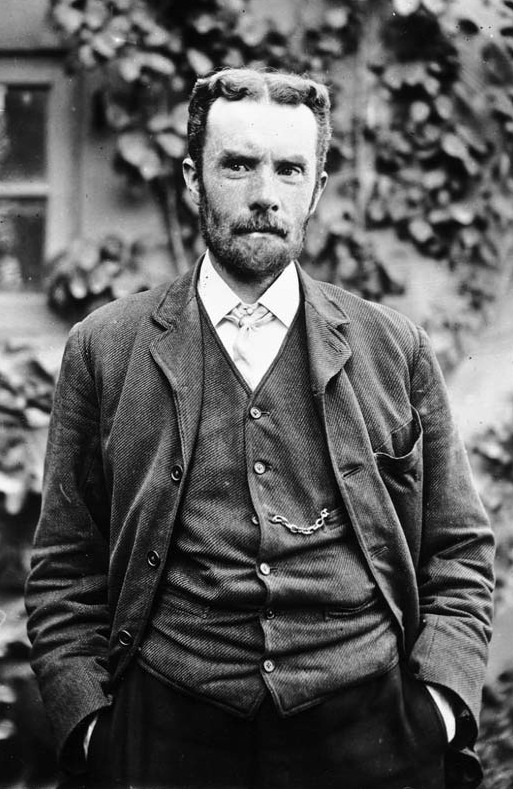
\includegraphics[scale=.10]{Oheaviside.jpg} \hspc  

	\[u_s(t) = \begin{cases} 
	      0 & t < 0 \\
	      1 & t\geq 0 \\
	   \end{cases}
	\]\\
	\[f_{step}(t) =Fu_s(t) 
		= \begin{cases} 
	      0 & t < 0 \\
	      F & t\geq 0 \\
	   \end{cases}
	\]\\

\end{multicols}

$u_s$ is the {\bf unit step function}  \vspc
$f_{step}$ is a step function of magnitude $F$ \vspc

}



% section 2: Obtaining the Response Equations in Problem 1

\section{T2: Obtaining the Response Equations in Problem 1}

\subsection{T2: Obtaining the Response Equations in Problem 1}
\frame{
\frametitle{T2: Obtaining the Response Equations in Problem 1}

You can see that each of the models in problem 1 is {\bf linear} and {\bf first order}. You do not have to re-derive (even though you could) the response equations but please reference where you found the equations you used. They are in the notes and in chapter 8. 



}

% section 3: Stability and the Roots

\section{T3: Finding the Time Value with Time Constant}

\subsection{T3: Finding the Time Value with Time Constant}
\frame{
\frametitle{T3: Finding the Time Value with Time Constant}

In problem b) it asks for the time at which the response equation reaches a certain value. There  are different ways to find this value.

\begin{itemize}
\item Plot the response curve and locate the value graphically. This might not be accurate.\vspc
\item Use a `root-finding' method to locate the value. \vspc
\item Solve for the value with algebra. This is easy for this system.\vspc
\end{itemize}

}

% section 3: Stability and the Roots

\section{T4: Stability of a Second Order System}

\subsection{T4: Stability of a Second Order System}
\frame{
\frametitle{T4: Stability of a Second Order System}


Our model  $m\ddot{x}+c\dot{x}+kx=0$ is stable if the roots of the characteristic equation lie {\it to the left} of the imaginary axis of the complex plane (if the Real part of the root is positive). This makes sense because a positive $\alpha$ would cause the response to go to $\infty$.\vspc

\begin{framed}
This is called the \textbf{Routh-Hurwitz stability conditions}\vspcc

A second order model of the form $a_2s^2+a_1s+a_0=0$ \vspc

if $a_2$, $a_1$, and $a_0$ have the {\it same sign}. \vspc
\end{framed}

This is in your reference handout and discussed on page 488 of System Dynamics, Palm III, Third Edition
}

% references is not a section for now, for looks and it would be a waste of space
\frame{

\frametitle{References}

\begin{itemize}
	\item System Dynamics, Palm III, Third Edition - Chapter 8 - System Response in the Time Domain
\end{itemize}

}
\end{document}









 